%--------------------------------------------------------------------
\titreTD{\thenumTD}{Les structures de Lewis}
%--------------------------------------------------------------------

\meth{L'algorithme de Lewis}

Rappeler les \'etapes pour construire une structure de Lewis, exemple du CO$_2$ 
(C central).
\begin{enumerate}[\bf {Étape} 1]
\item Dessiner le squelette $\sigma$ de la molécule.\\
\textsl{%
L'atome de carbone est central (il est donc entre les deux atomes d'oxygène)~:\\
\begin{figure}[h]
\centering 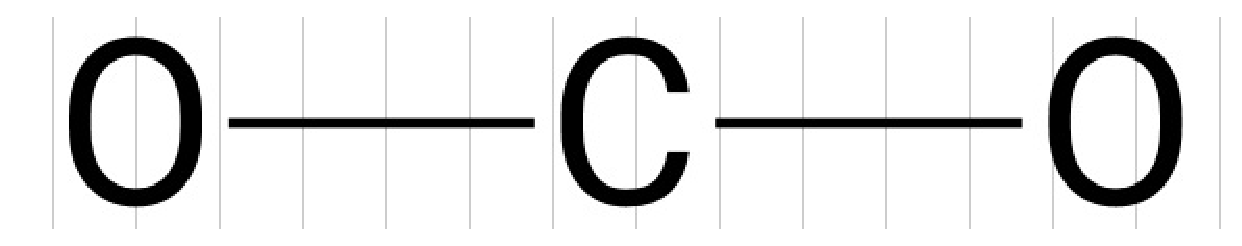
\includegraphics[height=1cm]{figure/CO2_01.eps}
\caption{\label{fig:squelette_de_co2}Squelette $\sigma$ de la molécule de CO$_2$.}
\end{figure}
}
\item Compter le nombre total d'électrons de valence, on appelle ce nombre $n_2$.\\
\textsl{%
La configuration électronique du carbone est $1s^22s^22p^2$, il apporte donc 4 électrons de
valence.
La configuration électronique de l'oxygène est $1s^2s^22p^4$, chaque atome d'oxygène apporte
donc 6 électrons de valence.
Donc~:
\begin{align*}
n_2 = 1\times 4 + 2\times 6 = 16
\end{align*}
}
\item Compléter la structure avec des doublets non liants pour que la règle de l'octet soit
respectée pour chaque atome.\\
\textsl{%
La règle de l'octet est respectée si chaque atome est entouré de 8 électrons.
Dans la figure \ref{fig:squelette_de_co2}, l'atome de carbone est entouré de 2 doublets, soit 4 électrons.
On lui ajout donc 2 doublets.
Dans cette même figure, les oxygènes sont entourés de 1 doublet (2 électrons), on leur ajoute donc
3 doublets.
Chaque atome est alors entouré de 8 électrons: la règle de l'octet est respectée.
\begin{figure}[h]
\centering 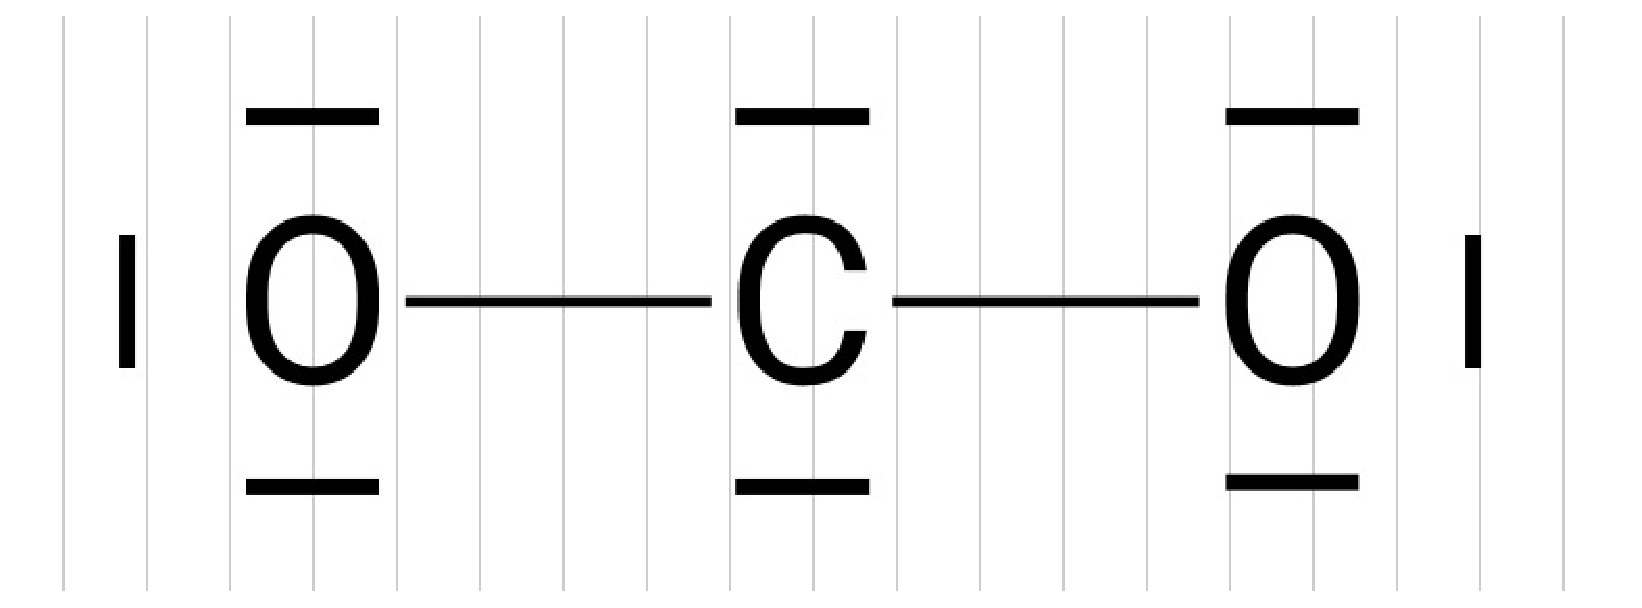
\includegraphics[height=2cm]{figure/CO2_02.eps}
\caption{\label{fig:octet_co2}Respect de la règle de l'octet. ATTENTION, ce n'est pas la
structure de Lewis finale!}
\end{figure}
}
\item Compter le nombre d'électrons dessinés. On appelle ce nombre $n_4$.
\begin{itemize}
\item si $n_4$>$n_2$ supprimer deux doublets non liants portés par deux atomes
adjacents et faire une liaison multiple entre ces atomes.
Repéter le processus jusqu'à ce que $n_4=n_2$.
\item sinon ajouter des doublets non liants sur les atomes hypervalents.
Repéter le processus jusqu'à ce que $n_4=n_2$.
\end{itemize}
\textsl{%
Dans la figure \ref{fig:octet_co2}, on a dessiné 10 doublets, soit 20 électrons ($n_4 = 20$).
Or $n_2=16$, donc $n_2<n_4$, on supprime donc deux doublets non liants portés par deux atomes
adjacents et on fait une liaison multiple entre ces atomes (voir figure \ref{fig:co2_1}).
\begin{figure}[h]
\centering 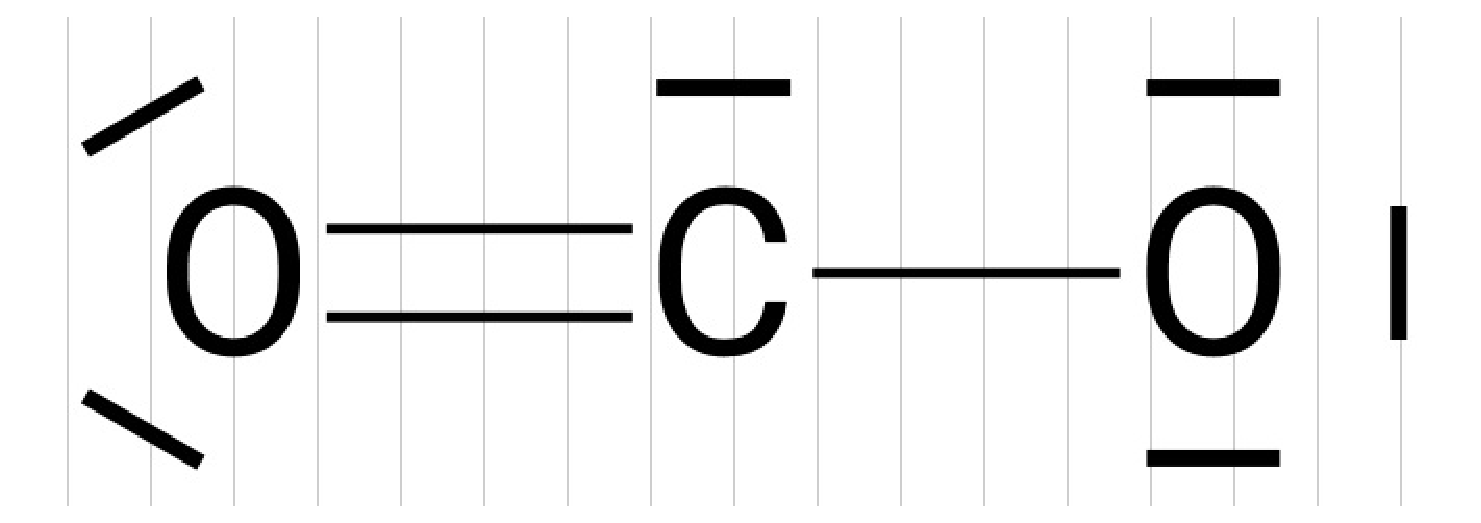
\includegraphics[height=2cm]{figure/CO2_031.eps}
\caption{\label{fig:co2_1}Dessin obtenu après avoir supprimé deux doublets non liants adjacents
et avoir créé une liaison multiple.}
\end{figure}
Comme dans la figure \ref{fig:co2_1}, $n_4=18$, on doit répéter le processus de suppression
de doublets et création de liaison multiple. On le fait de l'autre côté de la molécule
ce qui permet d'obtenir la figure \ref{fig:co2_1}.
\begin{figure}[h]
\centering 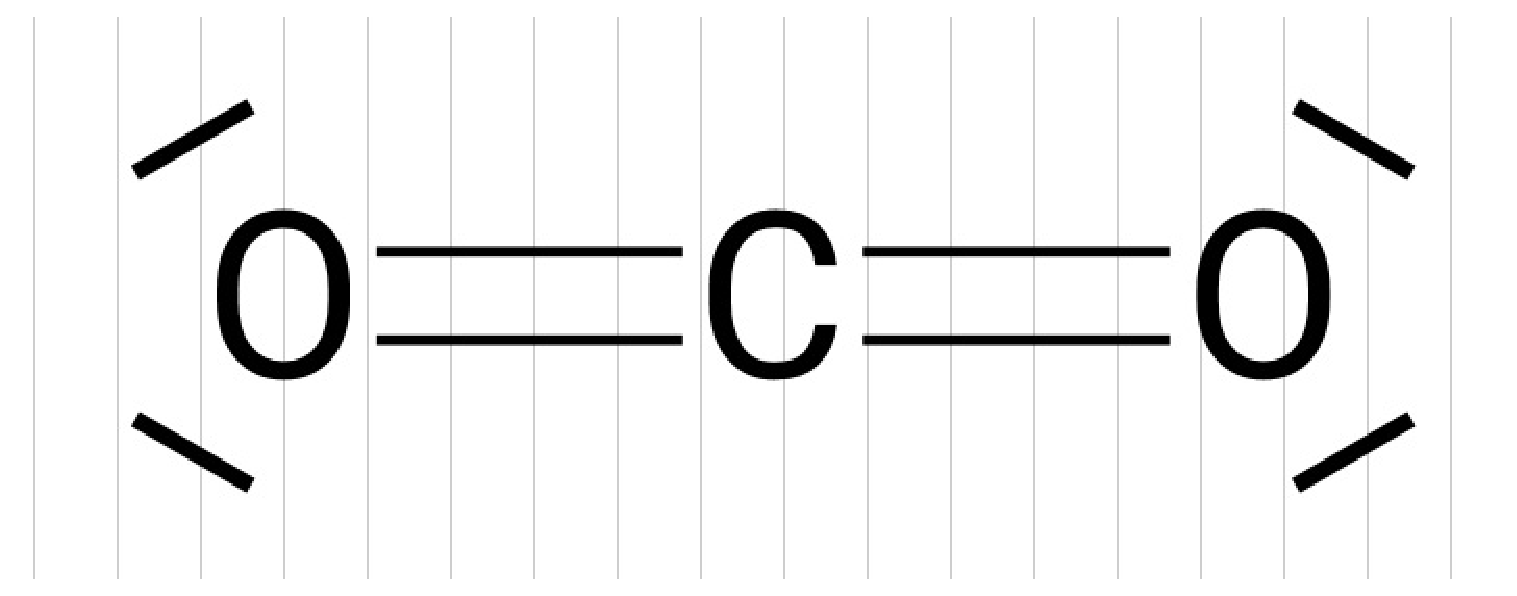
\includegraphics[height=2cm]{figure/CO2_032.eps}
\caption{\label{fig:co2_1}Dessin obtenu après avoir supprimé à nouveau deux doublets non liants adjacents
et avoir créé une liaison multiple.}
\end{figure}
}

\item Déterminer les charges formelles. Si deux charges opposées sont portées par deux atomes adjacents
et que l'un d'eux peut-être hypervalent, supprimer un doublet porté par l'atome chargé négativement
et faire une liaison multiple entre les deux atomes.
Repéter le processus autant que nécessaire.
\textsl{%
Pour déterminer les charges formelles de chaque atome, on casse les liaisons de manière
homolytique (la paire électronique est partagée entre les atomes).\\
\begin{figure}[h]
\centering 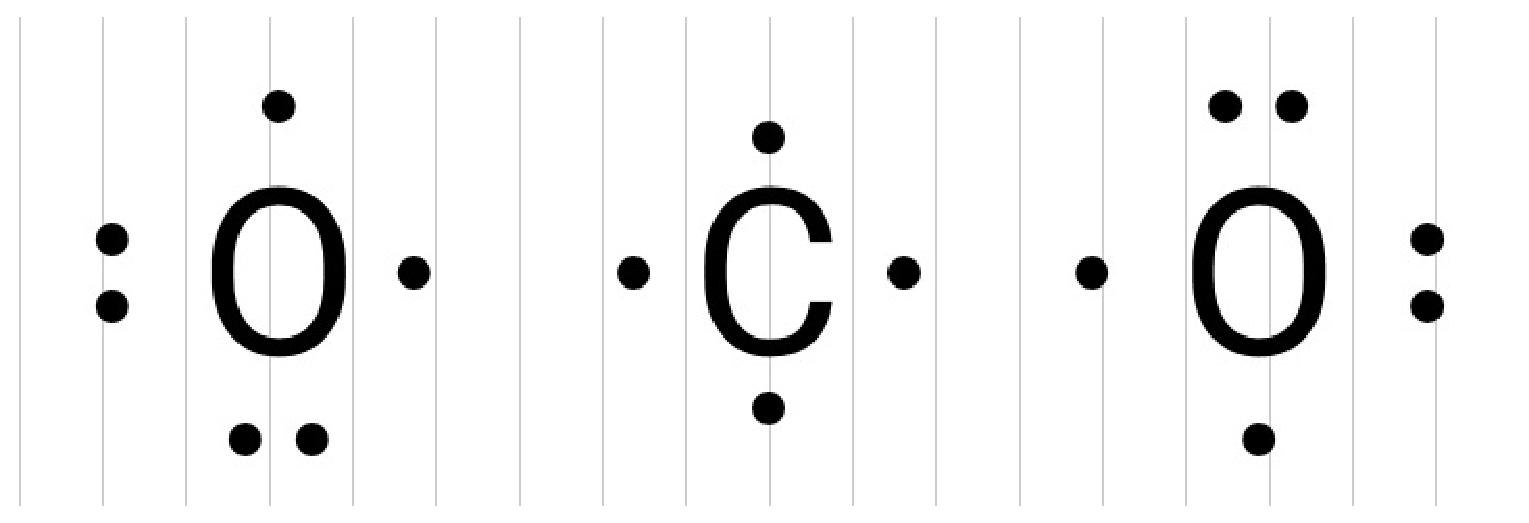
\includegraphics[height=2cm]{figure/CO2_04.eps}
\caption{\label{fig:co2_charges}Dessin utilisé pour le calcul des charges atomiques.}
\end{figure}
Pour l'atome de carbone on compte 4 électrons (voir figure \ref{fig:co2_charges}). Or cet atome a apporté 4 électrons de valence.
Il porte donc une charge de $4-4=0 \Rightarrow q_C=0$.
Pour les atomes d'oxygène on compte 6 électrons (voir figure \ref{fig:co2_charges}). Or ces atomes ont apporté 6 électrons de valence.
Ils portent donc chacun une charge de $6-6=0 \Rightarrow q_O=0$.
Il n'y a pas d'atomes adjacents portant des charges opposées, la structure de Lewis est donc:\\
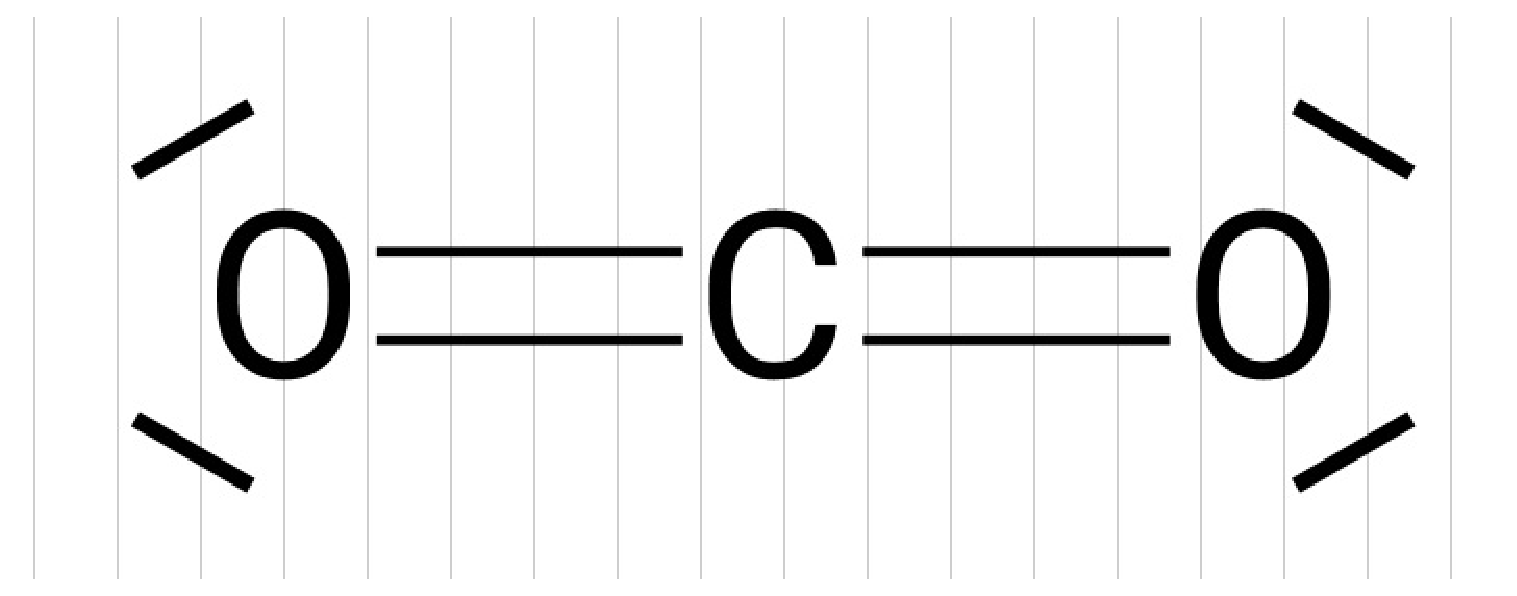
\includegraphics[height=2cm]{figure/CO2_032.eps}
}
\end{enumerate}

\exo{Structure de Lewis de mol\'ecules simples}

Pour chaque atome des compos\'es suivants  (diff\'erents de H), indiquer sa position dans 
le tableau p\'eriodique (p\'eriode et groupe). Compter les \'electrons de valence
et donner la structure de Lewis de chaque compos\'e. 
\'Etablir la charge de chaque atome.
%\'Etablir la charge et le degr\'e d'oxydation de chaque atome.

\begin{center}
\begin{tabular}{lll}
\hline                                           
H$_2$O      & HCN      & PCl$_3$                   \\
CH$_4$      & CH$_3$OH & CH$_3$CH$_3$              \\
NH$_3$      & HBr      & H$_2$S                    \\
NH$_2$OH    & SiH$_4$  & HCl                       \\
NF$_3$      & PH$_3$   & BH$_3$                    \\
\hline
\end{tabular}
\end{center}

\exo{Structures de Lewis et p\'eriode 3}

%Pour les syst\`emes suivants, \'etablir les structures de Lewis, la charge et le degr\'e
%d'oxydation de chaque atome. Quel est la particularit\'e des \'el\'ements P, Cl et S dans ces compos\'es~?
Pour les syst\`emes suivants, \'etablir les structures de Lewis et la charge de chaque atome.
Quel est la particularit\'e des \'el\'ements P, Cl et S dans ces compos\'es~?

{\small \textit{Pour construire le squelette de la mol\'ecule~: l'atome central est en gras et les atomes d'hydrog\`ene 
sont connect\'es aux atomes d'oxyg\`ene.}}

\vspace{0.5cm}

%\centerline{H$_3$\textbf{P}O$_4$, H$_3$\textbf{P}O$_2$, H$_2$\textbf{S}O$_4$, H\textbf{Cl}O, H\textbf{Cl}O$_4$.}
\centerline{H$_3$\textbf{P}O$_4$, H$_2$\textbf{S}O$_4$, H\textbf{Cl}O$_4$.}

%\exo{Structures de Lewis d'ions}
%
%Pour les syst\`emes suivants, \'etablir les structures de Lewis et la charge de chaque atome.
%
%\centerline{PF$_4^+$, CH$_3^+$, CH$_3^-$, NO$_2^-$}
%
%\exo{Structures de Lewis \'equivalentes} 
%
%Plusieurs structures de Lewis sont envisageables pour les mol\'ecules suivantes. 
%Les \'etablir pour chaque mol\'ecule. 
%
%\vspace{0.5cm}
%
%\centerline{NO$_2^-$, HNO$_3$, SO$_4^{2-}$, SO$_3$, HCO$_3^-$, CO$_3^{2-}$, ClO$_4^-$, O$_3$.}
%
